\subsection{Right-handed systems of vectors}

We begin with a discussion of right-handed systems of vectors in
$3$-dimensional
space.\index{right-handed system of vectors}\index{vector!right-handed system of}

\begin{definition}{Right-handed system of vectors}{right-hand}
  Three vectors, $\vect{u},\vect{v},\vect{w}$ form a right-handed
  system if when you extend the thumb of your right hand in the
  direction of $\vect{u}$ and your index finger in the direction of
  $\vect{v}$, your relaxed middle finger points roughly in the
  direction of $\vect{w}$.
  \begin{center}
    \raisebox{0.25in}{
      \begin{tikzpicture}
        \draw[->](0,0,0) -- node[right] {$\vect{u}$} (0,2,0);
        \draw[->](0,0,0) -- node[above] {$\vect{v}$} (-2,0,0);
        \draw[->](0,0,0) -- node[right] {$\vect{w}$} (0,0,3);
      \end{tikzpicture}
    }
    \hspace{1in}
    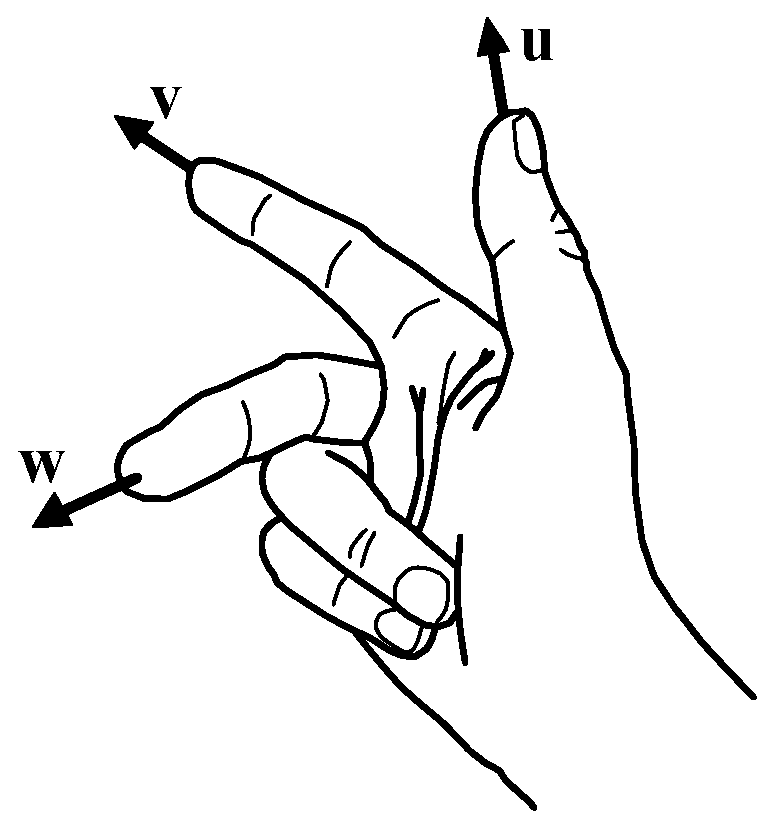
\includegraphics[height=1.8in]{figures/right-handed}
  \end{center}
\end{definition}

You should consider how a right-handed system would differ from a
left-handed system. Try using your left hand and you will see that the
vector $\vect{w}$ would need to point in the opposite direction.

Recall the special vectors $\vect{i}=\mat{1,0,0}^T$,
$\vect{j}=\mat{0,1,0}^T$, and $\vect{k}=\mat{0,0,1}^T$ we saw in
Section~\ref{sec:linear-combinations-rn}. We always assume that our
coordinate system is drawn in such a way that the vectors $\vect{i}$,
$\vect{j}$, $\vect{k}$ form a right-handed system. Thus, if the thumb
of your right hand points along the $x$-axis and your index finger
points along the $y$-axis, your middle finger should point along the
$z$-axis.

\begin{center}
\begin{tikzpicture}
\draw[->, thick] (0,0,0)--(2,0,0);
\draw[->, thick] (0,0,0)--(0,2,0);
\draw[->, thick] (0,0,0)--(0,0,2);
\node[below right] at (2,0,0){$\vect{j}$};
\node[below left] at (0,0,2){$\vect{i}$};
\node[above right] at (0,2,0){$\vect{k}$};
\end{tikzpicture}
\end{center}

\noindent
When all three vectors lie in a plane, then we say that the vectors
are \textbf{coplanar}%
\index{coplanar vectors}%
\index{vector!coplanar}. In this case, the system is neither
right-handed nor left-handed.
